\chapter{Evaluation} \label{chapter:EVALUATION}

We evaluated the functionality and practicability of our implementation.\\
For this, we used the setup described in the following section.


\section{Test Setup} \label{sec:EVALUATION:1}

We evaluated our implementation with the benchmark suite, the Lively Kernel version, and the machine configuration described in this section.

\subsection{The Octane Benchmark Suite}

% what?
We used the \emph{Octance} benchmark suite\footnote{\url{http://code.google.com/p/octane-benchmark/}, accessed February 3, 2014, at version 26} to evaluate the behavior and performance of our implementation.
Octane consists of eight JavaScript benchmarks.
It is a suite of real programs such as the \emph{DeltaBlue}~\cite{FreemanBenson1990ICS} constraint solver.
It does not test JavaScript's features systematically, but the benchmarks make use of many important language features, including primitive data types, operators, functions, objects, prototypical inheritance, and many built-in functions.\\
Octane is used for evaluating the performance of \emph{v8}, the engine used by Chrome and Node.js.
It is part of v8's official source code repository\footnote{\url{http://v8.googlecode.com/svn/}, accessed April 23, 2014, at revision 20901}.

% why?
We decided to use Octane for our evaluation for three reasons:

\begin{itemize}
    \item Octane is a standard benchmark suite.
    \item Octane covers many JavaScript language features.
    \item Octane is used in tuning Chrome's JavaScript engine and Chrome is the browser in which the Lively Kernel works best.
\end{itemize}


\subsection{The Lively Kernel}

% what?
During the implementation of our approach, we tested our prototype continuously with the Lively Kernel.

We developed our system in the Lively Kernel repository.
The commit we used for the evaluation is \emph{ed0586d80}\footnote{\url{http://github.com/LivelyKernel/LivelyKernel/commits/ed0586d80}, accessed May 9, 2014}. In this version, most of the Lively Kernel's code is passed through our transformations.
Only the Lively Kernel's bootstrap code, its module system, extensions to built-in types, and our implementation are excluded from the source transformations.
All modules loaded after these parts are transformed at load-time to enable versioning for them.
This includes, for example, all classes of the Lively Kernel.

% why?
We tested our implementation with the Lively Kernel for two reasons:

\begin{itemize}
    \item The Lively Kernel is a large JavaScript application that makes use of many features of the JavaScript language and the browser environment. The browser environment provides many built-in objects and functions. These are not part of the ECMAScript standard, but are nevertheless used by many applications. For example, the browser offers functions to manipulate its \ac{dom}, which the Lively Kernel uses for rendering. These built-ins are not covered by Octane or other popular JavaScript benchmark suites. 
    \item The goal of this work is to provide object versioning for the Lively Kernel. Thus, we are particularly interested in evaluating our implementation for the Lively Kernel.
\end{itemize}


\subsection{The Test Machine}

% what?
All tests and measurements were done on May 9, 2014 using a Macbook Air with a 2 GHz Intel Core i7 and 8 GB main memory, Mac OS X 10.9.2, and version 34.0.1847.131 of Chrome.

The presented measurement results were averaged over five runs.

% why?
We used Chrome for all experiments as the Lively Kernel currently works best in Chrome.



\section{Functionality of Version-aware References} \label{sec:EVALUATION:2}

We tested whether the version-aware references forward correctly to versions of objects with benchmarks and with the Lively Kernel.

\subsection{Testing with Benchmarks}

We ran the Octane benchmark suite to test the functionality of our implementation.

\paragraph{Method}
% what was done?
We transformed the Octane benchmarks with our source transformations, executed the resulting code, and then checked for JavaScript errors and compared the results of the transformed benchmarks to their usual results.\\
% why / to test what?
We did this to test two aspects.
First, to test whether our source transformations yield syntactically correct JavaScript code for the benchmarks.
Second, to test whether our proxy-based version-aware references, inserted by the source transformations, allow to run the benchmarks without errors and with the expected results.


\paragraph{Results}
All benchmarks in this suite run without errors and return the same results as when executed without any source transformations.
That is, at least for these tests, our source transformations produce working source code and our proxy-based version-aware references forward correctly to object versions.\\
During the development of our system, the \emph{DeltaBlue} benchmark revealed a problem when proxies are used as prototypes of objects.
We reported the issue to the \emph{harmony-reflect} repository\footnote{\url{http://github.com/tvcutsem/harmony-reflect/issues/18}, accessed April 23, 2014}.
The problem was identified as an issue with the \emph{v8} JavaScript engine\footnote{\url{http://code.google.com/p/v8/issues/detail?id=2804}, accessed April 23, 2014}.
We implemented a workaround for this problem, but the issue was subsequentely fixed, rendering the workaround redundant.

\paragraph{Discussion}
The proxies behave correctly like particular versions of objects in the situations tested by the benchmarks.
While these benchmarks do not test JavaScript's features systematically, they cover a wide range of important language features.


\subsection{Testing with the Lively Kernel}

We tested whether the Lively Kernel loads and works with our version-aware references.
Moreover, we tested whether versions of its state can be preserved with our implementation.

\paragraph{Method}
% what was done?
We transformed the JavaScript modules of the Lively Kernel at load-time to test whether it loads and works correctly with our proxy-based version-aware references.\\
Furthermore, we tested whether the system allows re-establishing versions of the Lively Kernel's state in practice.
Here, we tried multiple example scenarios, including to undo changes to the state and behavior of basic morphs, morph compositions, and the state of more complicated graphical applications as, for example, text editors and developer tools.\\
% why / to test what?
With this, we tested that the source transformations yield valid JavaScript code for the modules of the Lively Kernel, that the version-aware references delegate to the correct versions of objects, and that the version-aware references are used consistently.


\paragraph{Results}
The Lively Kernel loads when its modules are transformed to use our version-aware references.
Most of its basic functionality works as expected and we were able to preserve and re-establish runtime states of multiple examples.
However, not all functionality works as expected and we were, thus, not able to re-establish all preserved states.
In particular, we learned about the many built-in functions that currently do not handle proxies correctly in Chrome.
For this, we implemented the workaround described in Section~\ref{subsec:IMPLEMENTATION:4.3}.

\paragraph{Discussion}
Most of the tested functionality of the the Lively Kernel works correctly.
This includes the entire bootstrap process, rendering graphical objects, loading parts from the Lively Kernel's Parts Bin, and using the Lively Kernel's halo controls.
However, certain functionality of the Lively Kernel is not yet working correctly or even yields errors.
The remaining issues here are expected to be problems related to the built-in functions that do not work correctly when proxies are provided as arguments.
Our implementation already unwraps object versions from proxies for many built-in functions, as explained in Section~\ref{subsec:IMPLEMENTATION:4.3}, but the configuration does not cover all problematic built-in functions yet.\\
At the same time, the proxies are not yet fully supported by Chrome and we expect these issues not to be problematic anymore when proxies get fully implemented by Chrome's JavaScript engine.\\



\section{Practicability: Memory Consumption} \label{sec:EVALUATION:3}

We measured the memory overhead imposed by the version-aware references and how much memory is consumed when versions of the Lively Kernel's state are preserved.

For the measurements, we used Chrome's built-in memory profiler\footnote{\url{http://developers.google.com/chrome-developer-tools/docs/heap-profiling}, accessed May 8, 2014}.
It allows to take heap snapshots.
These snapshots contain all reachable JavaScript objects.
For each snapshot, Chrome shows the total size in megabyte.

\subsection{Memory Overhead of Version-aware References}

We measured how much more memory is required when loading the Lively Kernel with version-aware references.

\paragraph{Method}
% what was done?
We measured the memory required for loading a Lively Kernel world with and without version-aware references.
We took heap snapshots right after the world was completely loaded without interacting with the system.
We used an empty Lively Kernel world for this experiment and did not preserve any versions.
% why / to test what? 
% We decided to use an empty Lively Kernel world to measure the minimal overhead, while we expect the add to grow linearly with the number of proxied objects.

\paragraph{Results}
As shown in Figure~\ref{fig:MemoryOverheadForReferences}, loading an empty Lively Kernel world requires three times more space with proxies than without proxies.

\begin{figure}[h!]
    \centering
    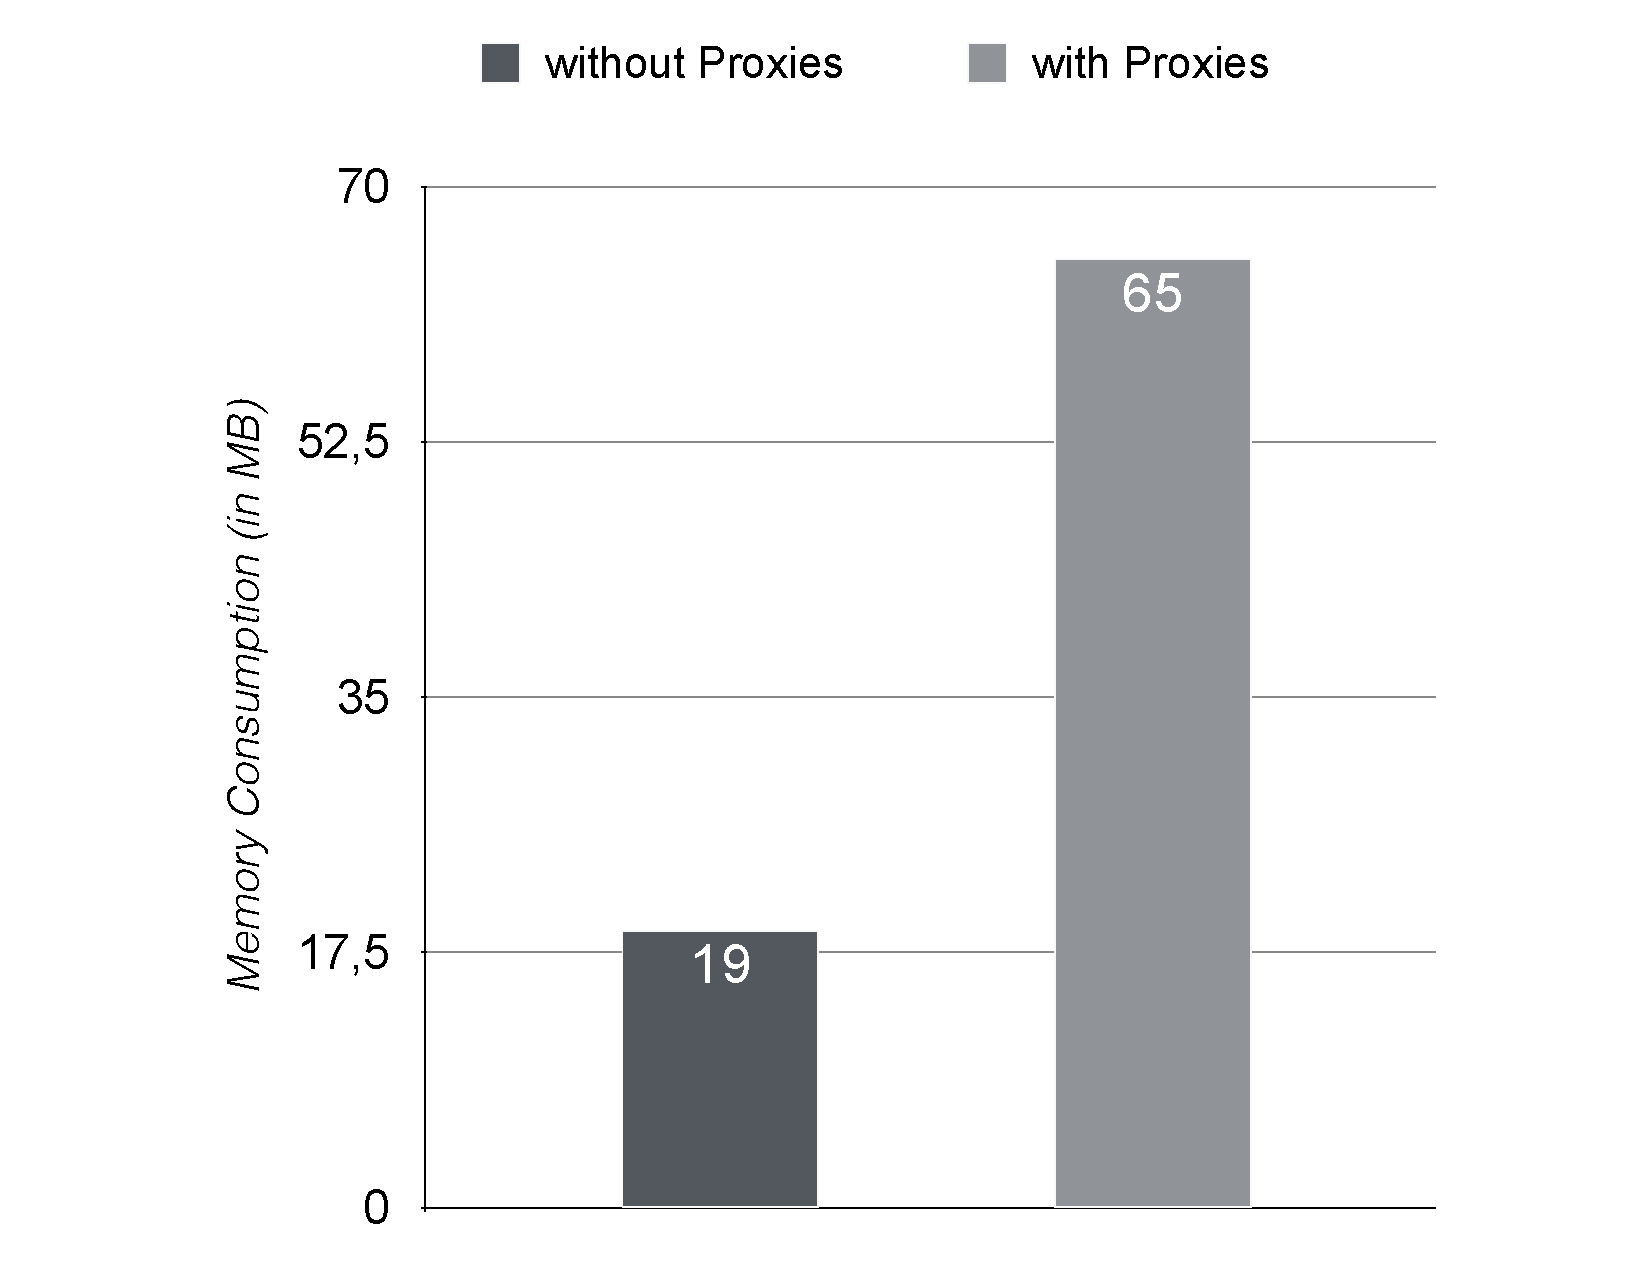
\includegraphics[width=0.7\textwidth]{figures/6_evaluation/1_memoryOverhead.pdf}
    \caption{Memory consumption when starting a Lively Kernel world with and without proxies.}
    \label{fig:MemoryOverheadForReferences}
\end{figure}

\paragraph{Discussion}
When loaded with proxies, the system requires space for the proxies.
Even without preserving multiple versions of any object, the system uses a proxy for each object.
These proxies require additional space: Each proxy comprises of at least a proxy object, a proxy handler object that specifies the proxy's behavior, and an object to hold all object versions.\\
We expect the memory overhead to increase linearly with the number of objects accessed through proxies.
While the system creates proxies for most objects, it does not use proxies for all objects.
In particular, it does not create proxies for objects that are present before our implementation of object versioning is loaded and all objects used by our implemenation itself.
We expect the number of objects that are excluded from versioning to be relatively stable.
All additional objects created at runtime will be accompanied by proxies.\\
% Currently, the proxies are not optimized to consume as little space as possible.
% Two improvements of the current implementation would be to not create a dictionary for managing multiple versions as long as a proxy stands-in for only one version and to have all proxy handler objects share their behavior.
% However, the memory overhead does not appear to be problematic at the moment.
The memory overhead does not appear to be problematic at the moment.


\subsection{Memory Used When Preserving Versions}

Besides the memory required for the version-aware references, memory is consumed when versions of the system are preserved.

\subsubsection{Method}
% what?
We measured how much memory is consumed when multiple versions of the system are preserved while working on a group of morphs.
The three states for which we took snapshots are shown as \circnum{1}, \circnum{2}, and \circnum{3} in the upper half of Figure~\ref{fig:MemoryOverheadForVersions}.
In particular, we did the following in this experiment:
\begin{enumerate}
    \item Version 1: We measured the memory consumed at State \circnum{1} in the initial version of the system.
    \item Version 2: We created a new version to preserve the initial state and then changed the state towards State \circnum{2} in the new version. Subsequentely, we measured the memory consumption for this state.
    \item Version 3: We preserved the previous state, changed the state to State \circnum{3} in a third version, and measured the memory consumption again.
\end{enumerate}

This experiment does not show how much memory is required exactly for storing multiple versions of particular objects.
Instead, the experiment shows the overall memory consumption of the entire Lively Kernel while our implementation is used realistically.

The snapshots include the size of all reachable JavaScript objects, not just the versions of the morph objects shown Figure~\ref{fig:MemoryOverheadForVersions}.
The reachable JavaScript objects in these snapshots are all objects of the Lively Kernel.
For example, the tools we used to change the morph states between the snapshots are implemented in JavaScript.
Their state is part of the system state.\\
We closed all tools before taking memory snapshots to exclude their state from the snapshots, but the Lively Kernel caches some state of these tools.
The cached state might be different in the three states.
Thus, the size of the cached state might be different in the three snapshots.
Moreover, previous versions of the cached state might be preserved with the versions of the system.

\subsubsection{Results}
Figure~\ref{fig:MemoryOverheadForVersions} shows the size of the three snapshots.
State \circnum{1} required the least memory.
State \circnum{2} requires 1.8 MB more memory.
It also requires 0.3 MB more memory than State \circnum{3}.

\begin{figure}[h!]
    \centering
    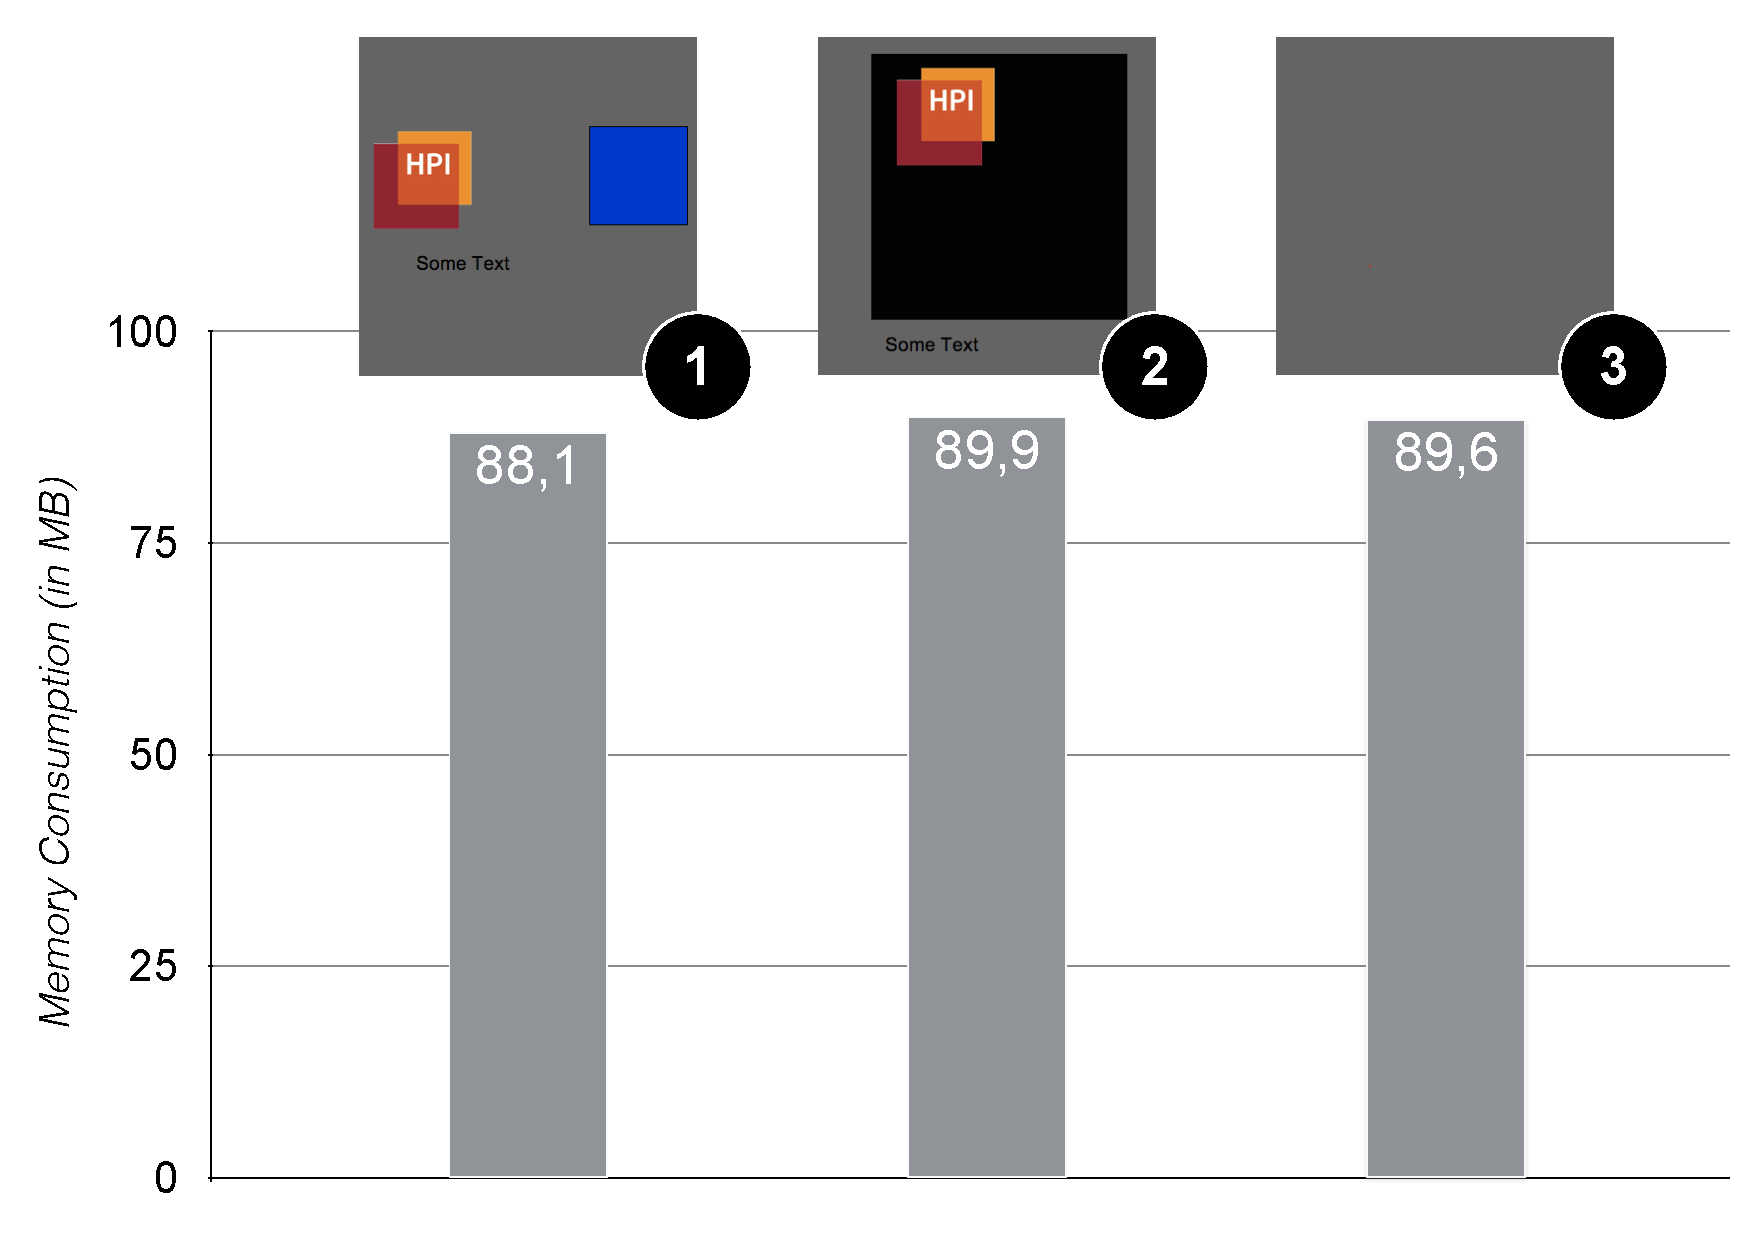
\includegraphics[width=0.76\textwidth]{figures/6_evaluation/2_memoryForVersions.pdf}
    \caption{Memory consumed for three different states when the previous states are preserved in separate versions.}
    \label{fig:MemoryOverheadForVersions}
\end{figure}

\subsubsection{Discussion}

The sizes of the three snapshots are not significantly different.
Even though it is not clear how much space is used for preserving the previous states of just the morphs, the results show that preserving system states requires relatively little memory.
Our implementation does not copy all objects for each version, but only creates copies when objects change from one version to another, effectively storing only the differences between system versions.
Therefore, the memory required for preserving versions of the system depends on how objects change in each version.
In the presented scenario, the space required for preserving the three states is insignificant to the space already required for running the Lively Kernel.

The results also show that the memory consumption does not always increase even when previous states are preserved: State \circnum{3} requires less memory than State \circnum{2}.
One explanation for this is that not all objects are preserved with the versions.
One category of such objects are the objects that only provide access to the elements of the browser's \ac{dom}, as described in \ref{subsubsec:DocumentModelProblem}.


\section{Practicability: Impact on Execution Speed} \label{sec:EVALUATION:4}

We measured the overhead our implementation of version-aware references imposes on running benchmarks and the Lively Kernel.
A discussion of the results follows at the end of this section.


\subsection{Running Benchmarks}

The Octane benchmark suite shows how the proxies currently slow down a variety of different JavaScript programs.\\
A microbenchmarks shows the specific cost of having proxies forward object interactions.

\subsubsection{Octane Benchmark Suite}

Measuring the Octane benchmark suite highlights how the execution of eight JavaScript programs is affected by the proxies.

\paragraph{Method}
We ran the Octane benchmarks\footnote{Note: We reduced the input size of the Splay benchmark by an order of magnitude to prevent the browser from prompting for user input during the benchmark's execution. The prompt is triggered due to the long time required to run the benchmark. It cannot be disabled and would influence the benchmark result.} with and without previous transformation of the benchmark code and, therefore, with or without version-aware references.
The source transformations for this were done separately before measuring the execution times.

\begin{figure}[h]
    \centering
    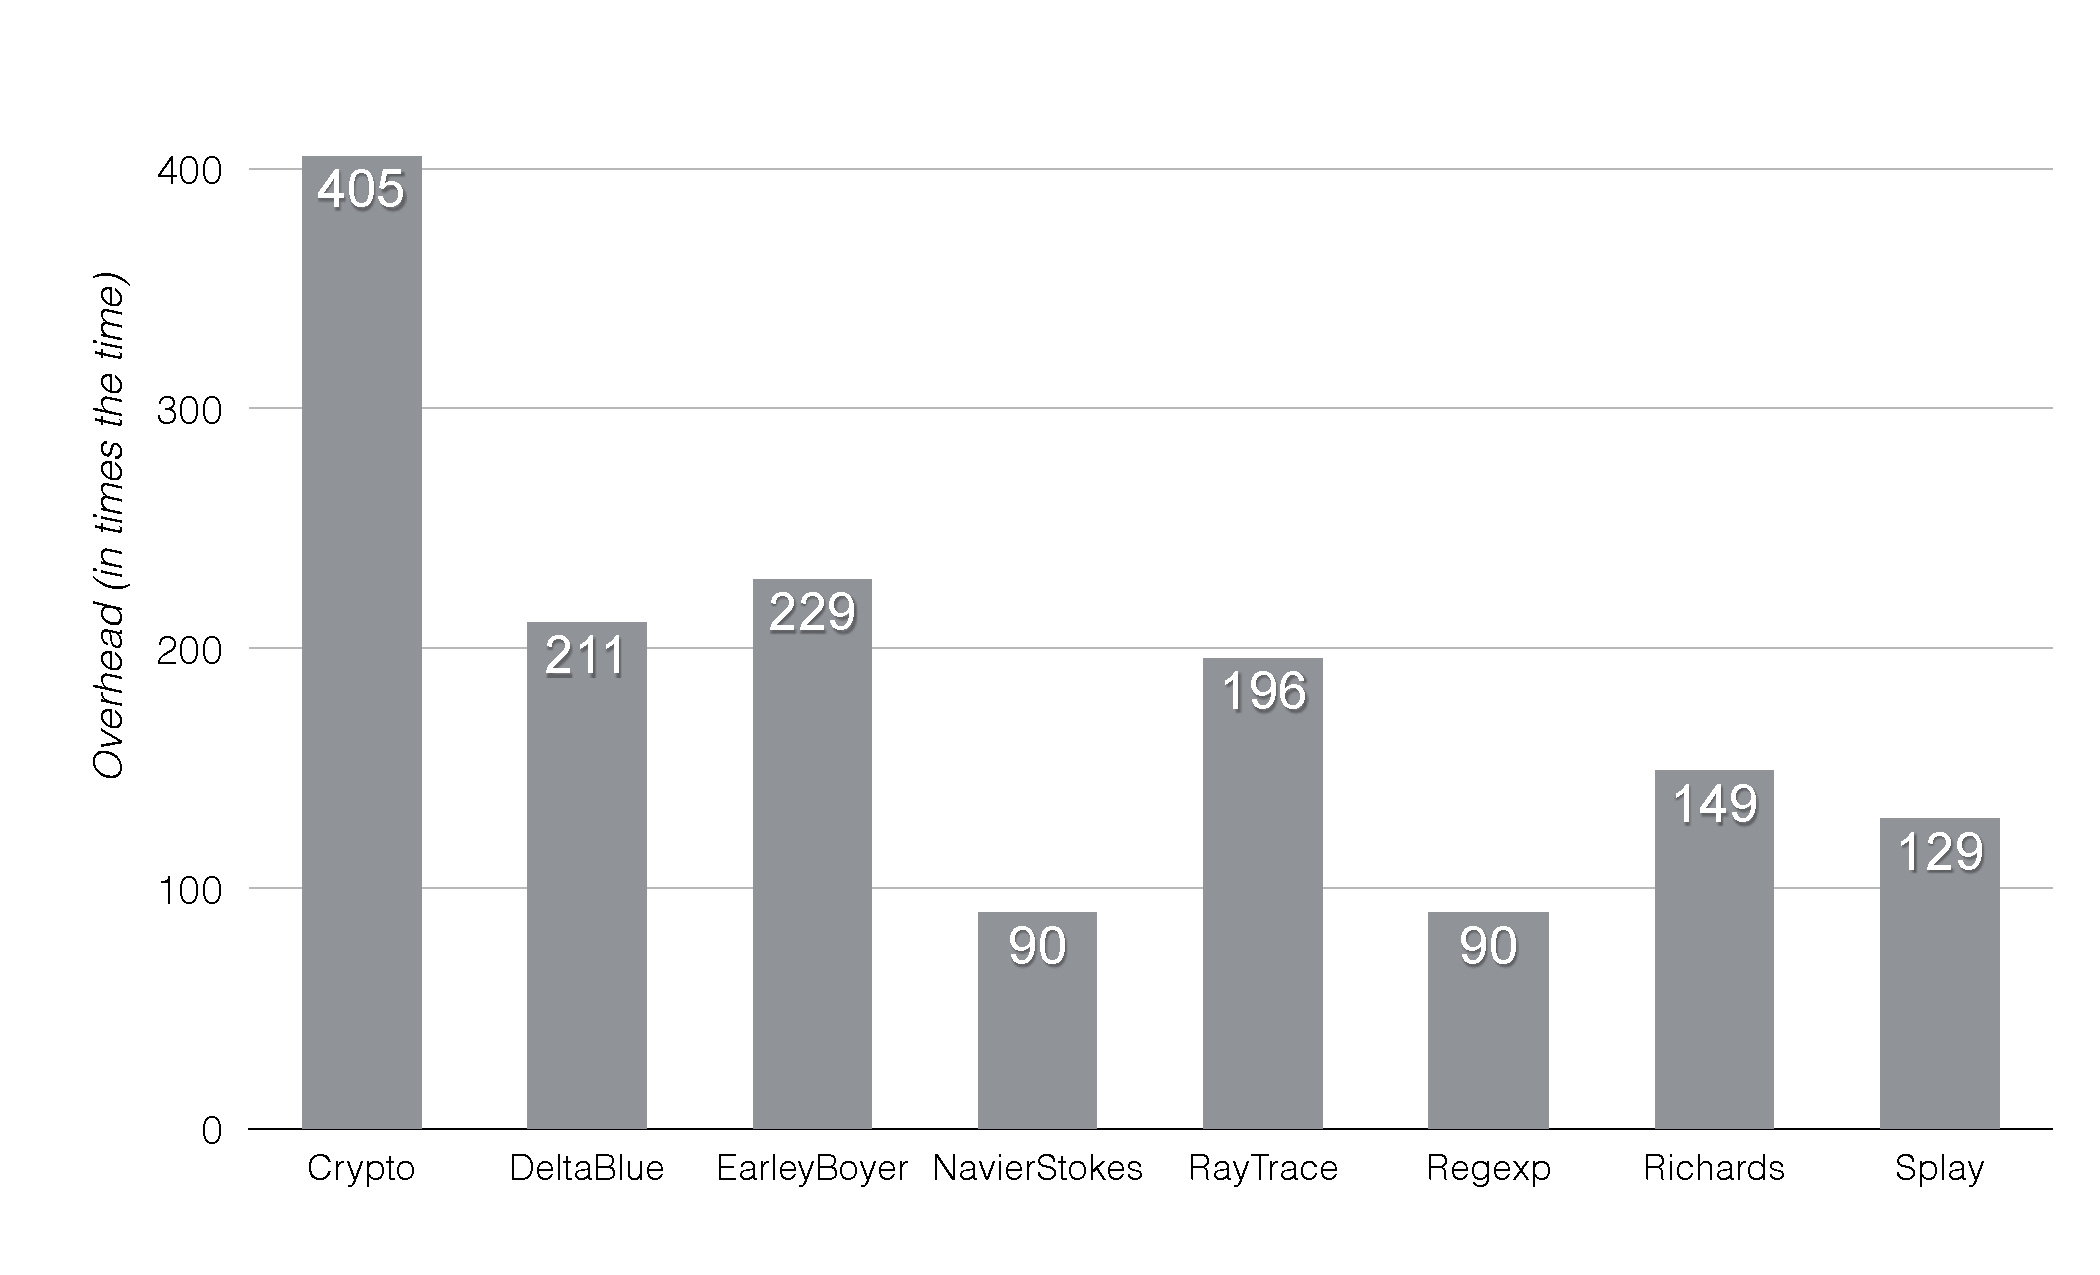
\includegraphics[width=\textwidth]{figures/6_evaluation/3_executionOverhead.pdf}
    \caption{Execution overhead of proxy-based version-aware references for the Octane benchmark suite.}
    \label{fig:ExecutionOverhead}
\end{figure}

\paragraph{Results}
Figure~\ref{fig:ExecutionOverhead} shows how much more time the benchmarks take when their source is transformed before execution and references are, therefore, version-aware.
Executing individual benchmarks takes between 90 and 405 times longer with version-aware references than without.
On average the execution is slowed down by a factor of 187.5.


\subsubsection{Microbenchmarks}

We implemented a microbenchmark to measure the overhead the proxies impose on resolving references.
In particular, the microbenchmark shows how much time the proxies require to intercept and forward property reads to the single version of an object.

\paragraph{Method}
% We resolved a reference that connects a \lstinline{client} object to a \lstinline{server} object a million times to read and call a function property.
We measured how long it takes to resolve a reference as well as read and call a function property a million times.
The reference connects a \lstinline{client} object to a \lstinline{server} object.
The code of which we measured the execution time is shown in Listing~\ref{lst:microbenchmark}.

\iffalse
\begin{verbatim}\fi
\begin{code}[lst:microbenchmark]{Code we measured for the microbenchmark.}{float}
for (var i=0; i < 1000000; i++) {
    client.server.foo();
} 
\end{code}
\iffalse
\end{verbatim}\fi

We compared the execution times of three different setups:

\begin{description}
    \item[Setup 1] The \lstinline{client} object holds a reference directly to the \lstinline{server}.
    \item[Setup 2] The \lstinline{client} object holds a proxy as its \lstinline{server} property. In this setup, we used the proxy handler described in Section~\ref{sec:IMPLEMENTATION:1} for the proxy. The proxy has access to the actual \lstinline{server} object as one of its version objects. It selects the \lstinline{server} object when it intercepts the property read.
    \item[Setup 3] The \lstinline{client} object's \lstinline{server} property is also a proxy but one created with a fixed target and without proxy handler. The fixed target is the \lstinline{server} object to which the proxy then forwards by default.
\end{description}

In all setups, the \lstinline{server} object holds a reference that directly refers to the \lstinline{foo} function.

% The \lstinline{client}'s reference is either an ordinary reference or version-aware.
% In the latter case, an ordinary reference refers from the \lstinline{client} to a proxy and that proxy forwards all object interactions to the \emph{server} object.\\
% In a first version of this setup, we provided the handler object described in \ref{sec:IMPLEMENTATION:1} when creating the proxy, so the proxy provides our versioning behavior: it has no fixed target object, but chooses the \lstinline{server} object dynamically following the global version identifier.\\
% In a second version of this microbenchmark, we provided no handler object when creating the proxy.
% In this case, the proxy falls back on the default proxy behavior, which is forwarding to a fixed target.
% The fixed target is the \lstinline{server} object.

\paragraph{Results}
Table~\ref{table:microbenchmarkResults} shows the results of running the microbenchmark in the three setups.
Using a proxy with our proxy handler takes three orders of magnitude more time than using an ordinary reference does: Instead of on average 10 milliseconds the test requires on average about 11000 milliseconds to finish.
The difference between \emph{Setup 3} and \emph{Setup 1} is an order of magnitude less: 2000 milliseconds compared to 10 milliseconds.
This shows, however, that even a proxy with a fixed target and the default proxy behavior slows down the execution of the microbenchmark close to 200 times.

\begin{table}[h]
\begin{center}
\begin{tabular}{| l | l |}
\hline
\emph{Setup 1} & 10 milliseconds \\ \hline
\emph{Setup 2} & 11000 milliseconds \\ \hline
\emph{Setup 3} & 2000 milliseconds \\ \hline
\end{tabular}
\end{center}
\caption[Table caption text]{Times to run the three setups of the microbenchmark.}
\label{table:microbenchmarkResults}
\end{table}

% In the first setup, the microbenchmark takes three orders of magnitude more time when the proxy is used to forward the property read to the \lstinline{server} object: instead of on average 10 milliseconds the test requires on average about 11000 milliseconds to finish.\\
% In the second setup, the difference is an order of magnitude less: with a direct reference the benchmark still requires around 10 milliseconds, but the benchmark requires requires close to 2000 milliseconds when the proxy forwards to its fixed target.
% That is, even the default proxy behavior slows down the microbenchmark close to 200 times.



\subsection{Execution of the Lively Kernel}

We measured the overhead imposed on three typical user interactions and how much longer it takes to load a Lively Kernel world with proxy-based version-aware references.

\subsubsection{Typical Lively Kernel Interactions}

As our goal is to provide recovery support for development in Lively Kernel, the overhead imposed on user interactions is especially interesting as it directly affects developers.

\paragraph{Method}
% what?
We measured the time three user interactions take when using proxies and compared this to the time the interactions usually take.
We measured the time from the user events until the single-threaded JavaScript engine becomes responsive again programmatically.
The three typical interaction we chose to investigate are: bringing up the halo buttons on a particular morph, opening the Lively Kernel's main menu, and opening the Lively Kernel's System Code Browser.\\
% why?
We chose these three interactions as we expect them to be more impacted by the version-aware references as, for example, interactions that are more browser-supported and less reliant on the execution of JavaScript code such as dragging elements around the screen.
All three interaction trigger code from multiple different modules, including event handling code, rendering code, and tool-specific code.

\begin{figure}[h!]
    \centering
    \includegraphics[width=0.8\textwidth]{figures/6_evaluation/4_LivelyInteractionsOverhead.pdf}
    \caption{Execution overhead for three user interactions in the Lively Kernel.}
    \label{fig:LivelyInteractionsOverhead}
\end{figure}

\paragraph{Results}
Figure \ref{fig:LivelyInteractionsOverhead} shows the results.
Each of the three interactions takes on average 43 times the time when triggered after the system was loaded with proxies.



\subsubsection{Loading a Lively Kernel World}

Another performance-related question specific to the Lively Kernel is how long it takes to load a world with proxies.

\paragraph{Method}
We measured how long it takes to load a specific Lively Kernel world with and without source transformations and, thus, proxies.
Loading a world includes requesting the required modules from the Lively Kernel's server, client-side code to resolve dependencies among those modules, evaluating the code of the loaded modules, and deserializing the graphical state of the world's scenegraph.
Additionally, in case proxies should be used, the sources of all modules also are transformed while loading the world.

\paragraph{Results}
It takes eight times more time to load a world with object versioning: instead of around 4 seconds, the user would have to wait around 32 seconds until the world becomes responsive.




\subsection{Discussion of the Execution Overhead}

The results of our evaluation show that the execution overhead is currently not practical.
The Octane benchmarks indicate that executing real JavaScript programs takes two to three orders of magnitude more time.
Similarly, the Lively Kernel tools are significantly less responsive.\\
Even though we expected a certain execution overhead with our approach, the current overhead is too high.

The microbenchmarks show that a considerable part of the overhead is introduced by using the ECMAScript 6 proxies.
Even when these proxies are used to forward to a fixed target instead of a dynamically chosen target, they introduce a substantial overhead:
It takes 200 times the time to have a proxy intercept and forward property reads than it takes to read a property after resolving an ordinary reference.\\
For this reason, we still consider our approach feasible for providing object versioning for the Lively Kernel.
The performance of our current implementation, however, needs to be improved before it provides practical recovery support to Lively Kernel programmers.







% oh boy, so much dead text..


% the results show a problem
% what exactly is the problem: proxies.. 
    % they do a lot of stuff
    % but also without providing a handler object, when all interactions with the proxy are just forwarded to a fixed target.. too much overhead
    
% --> need an alternative to proxies



% the proxies do a lot of stuff..

% inspecting the arguments, choosing the correct version to forward to, inspecting the result

% 
% When the proxies stand-in for the versions of an object, they intercept and forward all object interactions to a version.
% The proxies choose the version dynamically from a dictionary,
% In addition, before forwarding to a version, the proxies test whether the interaction requires special handling.
% 
% 
% 
% 




% While object versioning could be used to provide undo/redo for an application, it is primalary itented to support development.
% That could, conceivably, be an argument for providing object versioning only during development, not when programs are in-use and should run at full speed.
% Besides having the disadvantage of introducing distinct usage modes, this still requires the version-aware references to resolve fast enough to not impede development significantly, which they, currently, however, do.




% The microbenchmarks show that a significant overhead is introduced by using proxies for implementing version-aware references.
% The JavaScript proxies are part of an ECMAScript specification that has not yet been finalized.
% The current draft is not fully implemented by the JavaScript engines yet.
% As explained in Section~\ref{sec:IMPLEMENTATION:1}, the proxies are currently also implemented using a library that relies on an experimental implementation of a previous, deprecated draft of the proxy specification.
% 
% Similar behavior forwarding as provided by the proxy handlers could also be implemented in JavaScript, using source transformations and ordinary JavaScript functions.
% Instead of using an actual proxy for an object, we could have references point to an ordinary JavaScript object and implement the handler behavior in an ordinary JavaScript function, to be used through further source transformations: instead of \lstinline{obj.prop} the system would execute code similar to \lstinline{get(obj, \"name\")}, where the \lstinline{obj} could still be only a stand-in for many different versions, while \lstinline{get} could implement the behavior previously implemented by respective the proxy trap.
% Measuring the performance of such a simple indirection results in a much lower performance overhead for the previously described microbenchmark setup:
% it only takes twice the time to read a property from a specific target with a \lstinline{get}-function when compared to reading a property directly.
% 
% All this---the experimental status of the proxy implementation, the high cost of proxies even when used with the default handler behavior, and the significantly lower overhead of a custom indirection based on ordinary JavaScript functions---suggest that the performance of the ECMAScript 6 Direct Proxies in Chrome might improve in the future.
% At the same time, we might also decide to base our version-aware references on source transformations and custom indirections instead of proxies in the future.
% 
% 
% 
% While object versioning could be used to provide undo/redo for an application, it is primalary itented to support development.
% That could, conceivably, be an argument for providing object versioning only during development, not when programs are in-use and should run at full speed.
% Besides having the disadvantage of introducing distinct usage modes, this still requires the version-aware references to resolve fast enough to not impede development significantly.
% This is currently not the case.
% 
% The microbenchmarks show that a significant overhead is introduced by using proxies for implementing version-aware references.
% Version-aware references, however, could also be implemented in JavaScript using source transformations and ordinary JavaScript functions.
% Instead of \lstinline{obj.prop} the system could execute code similar to \lstinline{get(obj, \"name\")}.
% \lstinline{obj} could still be a stand-in for many versions of an object.
% \lstinline{get} could be a JavaScript function that .
% Measuring the performance of such a simple indirection results in a much lower performance overhead for the previously described microbenchmark setup:
% it only takes twice the time to read a property from a specific target with a \lstinline{get}-function when compared to reading a property directly.
